我们先简要介绍损失函数的概念，并说明链式法则如何方便地用于涉及张量与雅可比张量的表达式。损失函数 $L:S\times S\to \RR^{\geq 0}$ 用于度量计算模型、算法或决策过程在给出输出 $\hat{y}\in S$ 作为真值 $y\in S$ 的预测时所产生的误差或代价。许多学习与优化算法的目标就是最小化这一损失。一种做法是用 Frobenius 范数来度量预测输出与真值之差。当输入与输出都是张量时，可由雅可比张量算出所需梯度，从而最小化该 Frobenius 范数。设 $\At\in\RR^{d_1\times d_2\times d_3}$ 为真值，$\Tt\in\RR^{d_1\times d_2\times d_3}$ 为预测输出。利用定理~\ref{thm:gradients}，损失 $L = \norm{\At-\Tt}_F^2$ 的梯度可写为：
    \begin{align*}
        \frac{\partial\norm{\At-\Tt}_F^2}{\partial\Tt} 
        &=
        \frac{\partial}{\partial\Tt}\left(\norm{\At}_F^2 + \norm{\Tt}_F^2 - 2\langle\At,\Tt\rangle\right)\\
        &= 
    \frac{\partial}{\partial\Tt}\left(\begin{tikzpicture}[baseline=\baseline]
    \tikzset{tensor/.style = {minimum size = 0.5cm,shape = circle,thick,draw=black,inner sep = 0pt}, edge/.style = {thick,line width=.4mm},every loop/.style={}}
    \def\y{0}
    \def\x{0}
    \node[tensor,fill=green!50!red!50!white] (St) at (\x,\y){\scalebox{0.85}{$\Tt$}};
    \node[tensor,fill=green!50!red!50!white] (Tt) at (\x+1,\y){\scalebox{0.85}{$\Tt$}};
    \draw[edge] (St) -- (Tt);
    \draw[edge] (St) to [out=45,in=135] (Tt);
    \draw[edge] (St) to [out=-45,in=-135] (Tt);
    \node[draw=none] () at (\x+0.5,\y+0.5) {\scalebox{0.7}{\dimcolor{$d_1$}}};
    \node[draw=none] () at (\x+0.5,\y+0.15) {\scalebox{0.7}{\dimcolor{$d_2$}}};
    \node[draw=none] () at (\x+0.5,\y-0.5) {\scalebox{0.7}{\dimcolor{$d_3$}}};
\end{tikzpicture}
-2
~
\begin{tikzpicture}[baseline=\baseline]
    \tikzset{tensor/.style = {minimum size = 0.5cm,shape = circle,thick,draw=black,inner sep = 0pt}, edge/.style = {thick,line width=.4mm},every loop/.style={}}
    \def\y{0}
    \def\x{0}
    \node[tensor,fill=blue!40!red!20!white] (St) at (\x,\y){\scalebox{0.85}{$\At$}};
    \node[tensor,fill=green!50!red!50!white] (Tt) at (\x+1,\y){\scalebox{0.85}{$\Tt$}};
    \draw[edge] (St) -- (Tt);
    \draw[edge] (St) to [out=45,in=135] (Tt);
    \draw[edge] (St) to [out=-45,in=-135] (Tt);
    \node[draw=none] () at (\x+0.5,\y+0.5) {\scalebox{0.7}{\dimcolor{$d_1$}}};
    \node[draw=none] () at (\x+0.5,\y+0.15) {\scalebox{0.7}{\dimcolor{$d_2$}}};
    \node[draw=none] () at (\x+0.5,\y-0.5) {\scalebox{0.7}{\dimcolor{$d_3$}}};
\end{tikzpicture}
\right)\\
&=
\left(\begin{tikzpicture}[baseline=\baseline]
    \tikzset{tensor/.style = {minimum size = 0.5cm,shape = circle,thick,draw=black,inner sep = 0pt}, edge/.style = {thick,line width=.4mm},every loop/.style={}}
    \def\y{0}
    \def\x{0}
    \node[tensor,fill=green!50!red!50!white] (Tt) at (\x,\y){\scalebox{0.85}{$\Tt$}};
    \draw[edge](Tt) -- (\x+0.85,\y)node[midway, above]{\edgelabel{$d_2$}};
    \draw[edge](Tt) -- (\x-0.85,\y)node[midway, above]{\edgelabel{$d_1$}};
    \draw[edge](Tt) -- (\x,\y-0.85)node[midway, left]{\edgelabel{$d_3$}};
    \end{tikzpicture}
+
\begin{tikzpicture}[baseline=\baseline]
    \tikzset{tensor/.style = {minimum size = 0.5cm,shape = circle,thick,draw=black,inner sep = 0pt}, edge/.style = {thick,line width=.4mm},every loop/.style={}}
    \def\y{0}
    \def\x{0}
    \node[tensor,fill=green!50!red!50!white] (Tt) at (\x,\y){\scalebox{0.85}{$\Tt$}};
    \draw[edge](Tt) -- (\x+0.85,\y)node[midway, above]{\edgelabel{$d_2$}};
    \draw[edge](Tt) -- (\x-0.85,\y)node[midway, above]{\edgelabel{$d_1$}};
    \draw[edge](Tt) -- (\x,\y-0.85)node[midway, left]{\edgelabel{$d_3$}};
    \end{tikzpicture}
-2~~
\begin{tikzpicture}[baseline=\baseline]
    \tikzset{tensor/.style = {minimum size = 0.5cm,shape = circle,thick,draw=black,inner sep = 0pt}, edge/.style = {thick,line width=.4mm},every loop/.style={}}
    \def\y{0}
    \def\x{0}
    \node[tensor,fill=blue!40!red!20!white] (Tt) at (\x,\y){\scalebox{0.85}{$\At$}};
    \draw[edge](Tt) -- (\x+0.85,\y)node[midway, above]{\edgelabel{$d_2$}};
    \draw[edge](Tt) -- (\x-0.85,\y)node[midway, above]{\edgelabel{$d_1$}};
    \draw[edge](Tt) -- (\x,\y-0.85)node[midway, left]{\edgelabel{$d_3$}};
    \end{tikzpicture}\right)\\
&=
2\left(\begin{tikzpicture}[baseline=\baseline]
    \tikzset{tensor/.style = {minimum size = 0.5cm,shape = circle,thick,draw=black,inner sep = 0pt}, edge/.style = {thick,line width=.4mm},every loop/.style={}}
    \def\y{0}
    \def\x{0}
    \node[tensor,fill=green!50!red!50!white] (Tt) at (\x,\y){\scalebox{0.85}{$\Tt$}};
    \draw[edge](Tt) -- (\x+0.85,\y)node[midway, above]{\edgelabel{$d_2$}};
    \draw[edge](Tt) -- (\x-0.85,\y)node[midway, above]{\edgelabel{$d_1$}};
    \draw[edge](Tt) -- (\x,\y-0.85)node[midway, left]{\edgelabel{$d_3$}};
    \end{tikzpicture}
-
\begin{tikzpicture}[baseline=\baseline]
    \tikzset{tensor/.style = {minimum size = 0.5cm,shape = circle,thick,draw=black,inner sep = 0pt}, edge/.style = {thick,line width=.4mm},every loop/.style={}}
    \def\y{0}
    \def\x{0}
    \node[tensor,fill=blue!40!red!20!white] (Tt) at (\x,\y){\scalebox{0.85}{$\At$}};
    \draw[edge](Tt) -- (\x+0.85,\y)node[midway, above]{\edgelabel{$d_2$}};
    \draw[edge](Tt) -- (\x-0.85,\y)node[midway, above]{\edgelabel{$d_1$}};
    \draw[edge](Tt) -- (\x,\y-0.85)node[midway, left]{\edgelabel{$d_3$}};
    \end{tikzpicture}\right).
\end{align*}
链式法则很容易推广到涉及张量变量的表达式。例如，考虑任意损失函数 $\mathcal{ L}: \mathbb{R}^{d_1\times \cdots \times d_N} \to \mathbb{R}$，我们希望它在 $N$ 阶张量输入 $\Tt$ 上被最小化。再设该张量输入以张量网络的形式参数化，其中 $\Gt \in \mathbb{R}^{m_1\times \cdots \times m_M}$ 是一个 $M$ 阶核心张量。要计算 $\mathcal L$ 关于 $\Gt$ 的雅可比张量，可如下使用链式法则： 
$$\frac{\partial  \mathcal L}{\partial\Gt} 
=
\frac{\partial \mathcal L}{\partial \Tt }\frac{\partial\Tt}{\partial\Gt}  $$
其中 $\frac{\partial  \mathcal L}{\partial\Gt}$ 的尺寸为 $m_1\times\cdots \times m_M$，$\frac{\partial  \mathcal L}{\partial \Tt }$ 的尺寸为%
\footnote{严格来说，$\frac{\partial  \mathcal L}{\partial\Gt}$ 的形状为 $1\times m_1 \cdots \times m_M$，$\frac{\partial  \mathcal L}{\partial \Tt }$ 的形状为 $1\times d_1\times \cdots \times d_N$，只是维度为 $1$ 的第一个平凡模自然被省略了。}
$d_1\times \cdots \times d_N$，而 $\frac{\partial\Tt}{\partial\Gt} $ 的尺寸为 $d_1\times \cdots \times d_N \times m_1 \cdots \times m_M$。$\frac{\partial  \mathcal L}{\partial \Tt }$ 与 $\frac{\partial\Tt}{\partial\Gt}  $ 之间的乘积默认理解为：将 $\frac{\partial  \mathcal L}{\partial \Tt }$ 的 $M$ 个模与 $\frac{\partial\Tt}{\partial\Gt}  $ 的前 $M$ 个模相收缩。

有了这些工具，我们就可以用两个应用来结束本章，它们都涉及张量网络的梯度计算。 
\begin{itemize}
\item\textbf{用梯度下降求 CP 分解} 要求张量 $\Tt\in\RR^{d_1\times\cdots\times d_N}$ 的近似 CP 分解~(见第~\ref{sec:cp-decomposition}~节)，可用梯度下降最小化损失 $L = \norm{\Tt-\CP{\Gb_1,\cdots,\Gb_N}}^2_F$。这里 $\CP{\Gb_1,\cdots,\Gb_N}$ 表示 CP 分解，其中 $\Gb_1,\cdots,\Gb_N$ 为因子矩阵。为对因子矩阵作优化，可对损失函数施加梯度下降。例如在 $N=3$ 时，为求 $\Gb_1$，应用链式法则可写 $\frac{\partial L}{\partial\Gb_1} = \frac{\partial L}{\partial\CP{\Gb_1,\Gb_2,\Gb_3}}\frac{\partial\CP{\Gb_1,\Gb_2,\Gb_3}}{\partial\Gb_1}$，其中 $\frac{\partial L}{\partial\CP{\Gb_1,\Gb_2,\Gb_3}}= 2(\Tt-\CP{\Gb_1,\Gb_2,\Gb_3})\in\RR^{d_1\times d_2\times d_3}$，且 
\begin{align*}
\frac{\partial\CP{\Gb_1,\Gb_2,\Gb_3}}{\partial\Gb_1}
=
\begin{tikzpicture}[baseline=\baseline]
    \tikzset{tensor/.style = {minimum size = 0.5cm,shape = circle,thick,draw=black,inner sep = 0pt}, edge/.style   = {thick,line width=.4mm},every loop/.style={}}
    \def\y{0}
    \def\x{0}
 \node[tensor,fill=blue!50!white] (G2) at (\x+1,\y){$\Gb_2$};
   \node[tensor,fill=blue!20!white] (G3) at (\x+2,\y){$\Gb_3$};
    \draw  node[fill = black,circle,inner sep=0pt,minimum size=4pt] (m) at (\x+1,\y+1) {};
    \draw[edge] (m) -- (\x,\y+0.1) node [midway,left] {\edgelabel{$R$}};
    \draw[edge] (G2) -- (m)node [midway,left] {\edgelabel{$R$}};
    \draw[edge] (G3) -- (m)node [midway,right] {\edgelabel{$R$}};
    \draw[edge](\x,\y-0.1) -- (\x,\y-0.7) node [midway,right] {\edgelabel{$d_1$}};
    \draw[edge](G2) -- (\x+1,\y-0.7)node [midway,left] {\edgelabel{$d_2$}};
    \draw[edge](G3) -- (\x+2,\y-0.7) node [midway,left] {\edgelabel{$d_3$}};
\end{tikzpicture}\in\RR^{d_1\times d_2\times d_3\times R}.
\end{align*}
观察所得的张量网络可知，它能用矩阵化与 Khatri-Rao 积表示：
\begin{align*}
  \frac{\partial L}{\partial\Gb_1} 
&=
\frac{\partial L}{\partial\CP{\Gb_1,\Gb_2,\Gb_3}}\frac{\partial\CP{\Gb_1,\Gb_2,\Gb_3}}{\partial\Gb_1}\\
&=
\begin{tikzpicture}[baseline=-0.5ex]
    \tikzset{tensor1/.style = {minimum width = 3cm,minimum height = 0.6cm,shape = rounded rectangle,thick,draw=black,inner sep = 0pt}, edge/.style = {thick,line width=.4mm},every loop/.style={}}
     \tikzset{tensor2/.style = {minimum size = 0.5cm,shape = circle,thick,draw=black,inner sep = 0pt}, edge/.style   = {thick,line width=.4mm},every loop/.style={}}
    \def\y{1}
    \def\x{0}
    \node[tensor1,fill=blue!45!red!20!white] (Tt) at (\x,\y){$2(\Tt-\CP{\Gb_1,\Gb_2,\Gb_3})$};
    \node[tensor2,fill=blue!50!white] (G2) at (\x,\y-1){$\Gb_2$};
   \node[tensor2,fill=blue!20!white] (G3) at (\x+1,\y-1){$\Gb_3$};
    \draw  node[fill = black,circle,inner sep=0pt,minimum size=4pt] (m) at (\x+0.5,\y-1.85) {};
    \draw[edge](G2)--(m)node [midway,left] {\edgelabel{$R$}};
    \draw[edge](G3)--(m)node [midway,right] {\edgelabel{$R$}};    \draw[edge](Tt)--(G2)node [midway,left] {\edgelabel{$d_2$}};
    \draw[edge](\x+1,\y-0.3)--(G3)node [midway,left] {\edgelabel{$d_3$}};
    \draw[edge](m)--(\x+0.5,\y-2.25)node [midway,left] {\edgelabel{$R$}};
    \draw[edge](\x-0.75,\y-0.3) -- (\x-0.75,\y-2.25)node [midway,left] {\edgelabel{$d_1$}};
\end{tikzpicture}\\
&=\begin{tikzpicture}[baseline=-0.5ex]
    \tikzset{tensor/.style = {minimum width = 3cm,minimum height = 0.6cm,shape = rounded rectangle,thick,draw=black,inner sep = 0pt}, edge/.style = {thick,line width=.4mm},every loop/.style={}}
    \def\y{1}
    \def\x{0}
    \node[tensor,fill=blue!45!red!20!white] (Tt) at (\x,\y){$2(\Tt-\CP{\Gb_1,\Gb_2,\Gb_3})$};
    \node[tensor,fill=blue!25!red!45!white] (Gt) at (\x+1,\y-1){$\Gb_2\krao\Gb_3$};
    \draw[edge](\x+0.5,\y-0.3) -- (\x+0.5,\y-0.7);
    \draw[edge](\x+0.6,\y-0.3) -- (\x+0.6,\y-0.7)node [midway,right] {\edgelabel{$d_2d_3$}};
    \draw[edge](\x-0.75,\y-0.3) -- (\x-0.75,\y-2)node [midway,left] {\edgelabel{$d_1$}};
    \draw[edge](\x+0.85,\y-1.3) -- (\x+0.85,\y-2)node [midway,left] {\edgelabel{$R$}};
\end{tikzpicture}\\
&=
2(\Tt-\CP{\Gb_1,\Gb_2,\Gb_3})_{(1)}(\Gb_2\krao\Gb_3)
\in\RR^{d_1\times R}.
\end{align*}
 \item\textbf{机器学习} 为压缩神经网络，可用张量分解来参数化全连接层的稠密权重矩阵，从而减少内存占用~\citep{novikov2015tensorizing}。设 $\Wb\in\RR^{P\times D}$ 为权重矩阵，$\xb\in\RR^{D}$ 为神经网络某一层的输入向量。输出 $\yb\in\RR^{P}$ 由权重矩阵 $\Wb$ 与输入向量 $\xb$ 收缩而得。 
    设 $P = \Pi_{i=1}^N{p_i}$ 且 $D =\Pi_{i=1}^Nd_i$。将 $\Wb$ 与 $\xb$ 重排为张量后，便有
\begin{align*}
    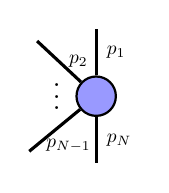
\begin{tikzpicture}[baseline=-0.1ex]
    \tikzset{tensor/.style = {minimum size = 0.5cm,shape = circle,thick,draw=black,inner sep = 0pt}, edge/.style = {thick,line width=.4mm},every loop/.style={}}
    \def\x{6}
    \def\y{0}
    \node[tensor,fill=blue!40!white] (y) at (\x,\y) {$\Yt$};
    \draw[edge](y)--(\x,\y+0.85)node [midway,right] {\scalebox{0.7}{\dimcolor{$p_1$}}};
    \draw[edge](y)--(\x-0.75,\y+0.7)node [midway,right=-0.01cm] {\scalebox{0.7}{\dimcolor{$p_2$}}};
    \draw[edge](y)--(\x-0.85,\y-0.7)node [very near end,right] {\scalebox{0.7}{\dimcolor{$p_{N-1}$}}};
    \draw[edge](y)--(\x,\y-0.85)node [midway,right] {\scalebox{0.7}{\dimcolor{$p_N$}}};
    \node[draw=none] at (\x-0.5,\y+0.1){$\vdots$};
    \end{tikzpicture}
=\sum_{d_1,\cdots,d_N}\Wt_{p_1,\cdots, p_N,d_1,\cdots, d_N}\Xt_{d_1,\cdots, d_N} =
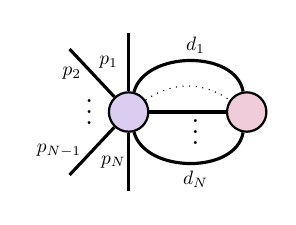
\begin{tikzpicture}[baseline=-0.1ex]
    \tikzset{tensor/.style = {minimum size = 0.5cm,shape = circle,thick,draw=black,inner sep = 0pt}, edge/.style = {thick,line width=.4mm},every loop/.style={}}
    \def\x{6}
    \def\y{0}
    \node[tensor,fill=red!30!blue!20!white] (w) at (\x,\y) {$\Wt$};
    \node[tensor,fill=blue!30!red!20!white] (x) at (\x+1.5,\y) {$\Xt$};
    \draw[edge](w)--(x);
    \draw[edge](w)--(\x,\y+1)node [midway,left] {\scalebox{0.7}{\dimcolor{$p_1$}}};
    \draw[edge](w)--(\x-0.75,\y+0.8)node [midway,left] {\scalebox{0.7}{\dimcolor{$p_2$}}};
    \draw[edge](w)--(\x-0.75,\y-0.8)node [midway,left] {\scalebox{0.7}{\dimcolor{$p_{N-1}$}}};
    \draw[edge](w)--(\x,\y-1)node [midway,left=-0.1cm] {\scalebox{0.7}{\dimcolor{$p_N$}}};
    \node[draw=none] at (\x-0.5,\y+0.1){$\vdots$};
   \draw[edge] (w) to [out=-75,in=-100] (x);
    \draw[edge] (w) to [out=75,in=100] (x);
    \draw[dotted] (w) to [out=35,in=145] (x);
    \node[draw=none] at (\x+0.85,\y-0.15){$\vdots$};
    \node[draw=none] () at (\x+0.85,\y+0.85) {\scalebox{0.7}{\dimcolor{$d_1$}}};
    (\x+1.2,\y-0.2){$\vdots$};
    \node[draw=none] () at (\x+0.85,\y-0.85) {\scalebox{0.7}{\dimcolor{$d_N$}}};
\end{tikzpicture}.
\end{align*}
为简单起见，下面只考虑 $N=4$ 的情形。文献~\citep{novikov2015tensorizing} 的作者提出以 MPO 格式参数化 $\Wt$~(见第~\ref{sec:efficient-operations}~节)，即 
$\Wt = 
\begin{tikzpicture}[baseline=\baseline]
    \tikzset{tensor/.style = {minimum size = 0.5cm,shape = circle,thick,draw=black,inner sep = 0pt}, edge/.style   = {thick,line width=.4mm},every loop/.style={}}
    \def\y{0}
    \def\x{0}
  \node[tensor,fill=red!30!white] (G1) at (\x,\y){$\Gt_1$};
  \node[tensor,fill=red!50!white] (G2) at (\x+1,\y){\scalebox{0.85}{$\Gt_2$}};
  \node[tensor,fill=blue!30!white] (G3) at (\x+2,\y){$\Gt_3$};
  \node[tensor,fill=blue!50!white] (G4) at (\x+3,\y){$\Gt_4$};
    \draw[edge](G1) -- (\x,\y-0.85)node [midway,left] {\edgelabel{$d_1$}};
    \draw[edge](G2) -- (\x+1,\y-0.85)node [midway,left] {\edgelabel{$d_2$}};
     \draw[edge](G3) -- (\x+2,\y-0.85)node [midway,left] {\edgelabel{$d_3$}};
    \draw[edge](G4) -- (\x+3,\y-0.85)node [midway,left] {\edgelabel{$d_4$}};
    \draw[edge](G1) -- (G2) node [midway,above] {\edgelabel{$R_1$}};
    \draw[edge](G2) -- (G3) node [midway,above] {\edgelabel{$R_2$}};
    \draw[edge](G3) -- (G4) node [midway,above] {\edgelabel{$R_3$}};
    \draw[edge](G1) -- (\x,\y+0.85)node [midway,left] {\edgelabel{$p_1$}};
    \draw[edge](G2) -- (\x+1,\y+0.85)node [midway,left] {\edgelabel{$p_2$}};
    \draw[edge](G3) -- (\x+2,\y+0.85)node [midway,left] {\edgelabel{$p_3$}};
    \draw[edge](G4) -- (\x+3,\y+0.85)node [midway,left] {\edgelabel{$p_4$}};
\end{tikzpicture}.$
在反向传播步骤中，由于要更新的是权重矩阵，就需要对全部核心张量作优化。按链式法则，对 $i\in[4]$ 有 $\frac{\partial L}{\partial \Gt_i} = \frac{\partial L}{\partial \Yt}\frac{\partial\Yt}{\partial\Gt_i}$，其中 $L$ 表示损失函数。例如 $i=2$ 时，需求 $\Yt$ 关于 $\Gt_2$ 的导数。利用定理~\ref{thm:gradients}，只需从张量网络中删去 $\Gt_2$ 便可得到结果：
\begin{align*}
\frac{\partial\Yt}{\partial\Gt_2} 
&=
\frac{\partial\left(\begin{tikzpicture}[baseline=\baseline]
    \tikzset{tensor/.style = {minimum size = 0.5cm,shape = circle,thick,draw=black,inner sep = 0pt}, edge/.style   = {thick,line width=.4mm},every loop/.style={}}
    \def\y{0}
    \def\x{0}
  \node[tensor,fill=red!30!white] (G1) at (\x,\y){$\Gt_1$};
  \node[tensor,fill=red!50!white] (G2) at (\x+1,\y){\scalebox{0.85}{$\Gt_2$}};
  \node[tensor,fill=blue!30!white] (G3) at (\x+2,\y){$\Gt_3$};
  \node[tensor,fill=blue!50!white] (G4) at (\x+3,\y){$\Gt_4$};
  \node[tensor,fill=blue!30!red!20!white] (x) at (\x+1.5,\y-1.5) {$\Xt$};
    \draw[edge](G1) -- (\x,\y-0.85)node [midway,left] {\edgelabel{$d_1$}};
    \draw[edge](x)--(\x,\y-0.85);
    \draw[edge](G2) -- (\x+1,\y-0.85)node [midway,left] {\edgelabel{$d_2$}};
    \draw[edge](x)--(\x+1,\y-0.85);
     \draw[edge](G3) -- (\x+2,\y-0.85)node [midway,left] {\edgelabel{$d_3$}};
    \draw[edge](x)--(\x+2,\y-0.85);
    \draw[edge](G4) -- (\x+3,\y-0.85)node [midway,left] {\edgelabel{$d_4$}};
    \draw[edge](x)--(\x+3,\y-0.85);
    \draw[edge](G1) -- (G2) node [midway,above] {\edgelabel{$R_1$}};
    \draw[edge](G2) -- (G3) node [midway,above] {\edgelabel{$R_2$}};
    \draw[edge](G3) -- (G4) node [midway,above] {\edgelabel{$R_3$}};
    \draw[edge](G1) -- (\x,\y+0.85)node [midway,left] {\edgelabel{$p_1$}};
    \draw[edge](G2) -- (\x+1,\y+0.85)node [midway,left] {\edgelabel{$p_2$}};
    \draw[edge](G3) -- (\x+2,\y+0.85)node [midway,left] {\edgelabel{$p_3$}};
    \draw[edge](G4) -- (\x+3,\y+0.85)node [midway,left] {\edgelabel{$p_4$}};
\end{tikzpicture}\right)}{\partial\Gt_2}\\
&=
\begin{tikzpicture}[baseline=\baseline]
    \tikzset{tensor/.style = {minimum size = 0.5cm,shape = circle,thick,draw=black,inner sep = 0pt}, edge/.style   = {thick,line width=.4mm},every loop/.style={}}
    \def\y{-1}
    \def\x{0}
  \node[tensor,fill=red!30!white] (G1) at (\x,\y+1.5){$\Gt_1$};
    \node[tensor,fill=blue!30!white] (G3) at (\x+2,\y+1.5){$\Gt_3$};
  \node[tensor,fill=blue!50!white] (G4) at (\x+3,\y+1.5){$\Gt_4$};
  \node[tensor,fill=blue!30!red!20!white] (x) at (\x+1.5,\y) {$\Xt$};
    \draw[edge](G1) -- (\x,\y+0.85)node [midway,left] {\edgelabel{$d_1$}};
    \draw[edge](x)--(\x,\y+0.85);
    \draw[edge](\x+1,\y+1.35) -- (\x+1,\y+0.85)node [midway,left] {\edgelabel{$d_2$}};
    \draw[edge](x)--(\x+1,\y+0.85);
     \draw[edge](G3) -- (\x+2,\y+0.85)node [midway,left] {\edgelabel{$d_3$}};
    \draw[edge](x)--(\x+2,\y+0.85);
    \draw[edge](G4) -- (\x+3,\y+0.85)node [midway,left] {\edgelabel{$d_4$}};
    \draw[edge](x)--(\x+3,\y+0.85);
    \draw[edge](G3) -- (G4) node [midway,above] {\edgelabel{$R_3$}};
    \draw[edge](G1) -- (\x,\y+2.35)node [midway,left] {\edgelabel{$p_1$}};
    \draw[edge](G3) -- (\x+2,\y+2.35)node [midway,left] {\edgelabel{$p_3$}};
    \draw[edge](G4) -- (\x+3,\y+2.35)node [midway,left] {\edgelabel{$p_4$}};
    \draw[edge](G1)--(\x+0.85,\y+1.5) node [midway,above] {\edgelabel{$R_1$}};
    \draw[edge](G3)--(\x+1.25,\y+1.5) node [midway,above] {\edgelabel{$R_2$}};
    \draw[edge](\x+1,\y+1.6)--(\x+1,\y+2.35) node [midway,left] {\edgelabel{$p_2$}};
\end{tikzpicture}\in\RR^{p_1\times R_1\times p_2\times R_2\times p_3\times p_4\times d_2}.
\end{align*}
于是损失的梯度为
\begin{align*}
    \frac{\partial L}{\partial\Gt_2} = \frac{\partial L}{\partial\Yt}\frac{\partial \Yt}{\partial\Gt_2}
    =
    \begin{tikzpicture}[baseline=\baseline]
    \tikzset{tensor/.style = {minimum size = 0.5cm,shape = circle,thick,draw=black,inner sep = 0pt}, edge/.style   = {thick,line width=.4mm},every loop/.style={}}
    \def\y{-1.5}
    \def\x{0}
    \node[tensor,fill=green!30!white] (L) at (\x+1.5,\y+3.25){$\frac{\partial L}{\partial\Yt}$};
  \node[tensor,fill=red!30!white] (G1) at (\x,\y+1.5){$\Gt_1$};
    \node[tensor,fill=blue!30!white] (G3) at (\x+2,\y+1.5){$\Gt_3$};
  \node[tensor,fill=blue!50!white] (G4) at (\x+3,\y+1.5){$\Gt_4$};
  \node[tensor,fill=blue!30!red!20!white] (x) at (\x+1.5,\y) {$\Xt$};
    \draw[edge](G1) -- (\x,\y+0.85)node [midway,left] {\edgelabel{$d_1$}};
    \draw[edge](x)--(\x,\y+0.85);
    \draw[edge](\x+1,\y+1.35) -- (\x+1,\y+0.85)node [midway,left] {\edgelabel{$d_2$}};
    \draw[edge](x)--(\x+1,\y+0.85);
     \draw[edge](G3) -- (\x+2,\y+0.85)node [midway,left] {\edgelabel{$d_3$}};
    \draw[edge](x)--(\x+2,\y+0.85);
    \draw[edge](G4) -- (\x+3,\y+0.85)node [midway,left] {\edgelabel{$d_4$}};
    \draw[edge](x)--(\x+3,\y+0.85);
    \draw[edge](G3) -- (G4) node [midway,above] {\edgelabel{$R_3$}};
    \draw[edge](G1) -- (\x,\y+2.35)node [midway,left] {\edgelabel{$p_1$}};
    \draw[edge](L)--(\x,\y+2.35);
    \draw[edge](G3) -- (\x+2,\y+2.35)node [midway,left] {\edgelabel{$p_3$}};
    \draw[edge](L)--(\x+2,\y+2.35);
    \draw[edge](G4) -- (\x+3,\y+2.35)node [midway,left] {\edgelabel{$p_4$}};
    \draw[edge](L)--(\x+3,\y+2.35);
    \draw[edge](G1)--(\x+0.85,\y+1.5) node [midway,above] {\edgelabel{$R_1$}};
    \draw[edge](G3)--(\x+1.25,\y+1.5) node [midway,above] {\edgelabel{$R_2$}};
    \draw[edge](\x+1,\y+1.6)--(\x+1,\y+2.35) 
    node [midway,left] {\edgelabel{$p_2$}};
    \draw[edge](L)--(\x+1,\y+2.35);
\end{tikzpicture}\in\RR^{R_1\times p_2\times R_2\times d_2}.
\end{align*}

\end{itemize}






